%%%%%%%%%%%%%%%%%%%%%%%%%%%%%%%%%%%%%%%%%
% Class Notes Template
% LaTeX Template
% By: Ryan Grove
%%%%%%%%%%%%%%%%%%%%%%%%%%%%%%%%%%%%%%%%%

%----------------------------------------------------------------------------------------
%	PACKAGES AND OTHER DOCUMENT CONFIGURATIONS
%----------------------------------------------------------------------------------------

\documentclass[paper=a4, fontsize=11pt]{scrartcl} % A4 paper and 11pt font size

\usepackage[T1]{fontenc} % Use 8-bit encoding that has 256 glyphs
\usepackage{fourier} % Use the Adobe Utopia font for the document - comment this line to return to the LaTeX default
\usepackage[english]{babel} % English language/hyphenation
\usepackage{amsmath,amsfonts,amsthm} % Math packages

\usepackage{lipsum} % Used for inserting dummy 'Lorem ipsum' text into the template

\usepackage{sectsty} % Allows customizing section commands
\allsectionsfont{\centering \normalfont\scshape} % Make all sections centered, the default font and small caps

\usepackage{fancyhdr} % Custom headers and footers
\pagestyle{fancyplain} % Makes all pages in the document conform to the custom headers and footers
\fancyhead{} % No page header - if you want one, create it in the same way as the footers below
\fancyfoot[L]{} % Empty left footer
\fancyfoot[C]{} % Empty center footer
%\fancyfoot[R]{\thepage} % Page numbering for right footer
\renewcommand{\headrulewidth}{0pt} % Remove header underlines
\renewcommand{\footrulewidth}{0pt} % Remove footer underlines
\setlength{\headheight}{13.6pt} % Customize the height of the header

\numberwithin{equation}{section} % Number equations within sections (i.e. 1.1, 1.2, 2.1, 2.2 instead of 1, 2, 3, 4)
\numberwithin{figure}{section} % Number figures within sections (i.e. 1.1, 1.2, 2.1, 2.2 instead of 1, 2, 3, 4)
\numberwithin{table}{section} % Number tables within sections (i.e. 1.1, 1.2, 2.1, 2.2 instead of 1, 2, 3, 4)

\setlength\parindent{0pt} % Removes all indentation from paragraphs - comment this line for an assignment with lots of text

\usepackage{lastpage}
\usepackage{fancyhdr}
\cfoot{\thepage\ of \pageref{LastPage}}

\def\v{\hbox{$\mathbf v$}}
\def\w{\hbox{$\mathbf w$}}
\def\u{\hbox{$\mathbf u$}}
\def\x{\hbox{$\textbf{x}$}}
\def\z{\hbox{$\mathbf z$}}
\def\a{\hbox{$\mathbf a$}}
\def\b{\hbox{$\mathbf b$}}
\def\L{\hbox{$\mathcal L$}}
\def\C{\hbox{$\mathbb C$}}
\def\B{\hbox{$\mathcal B$}}
\def\R{\hbox{$\mathbb R$}}
\def\X{\hbox{$\underline X$}}
\def\Q{\hbox{$\mathbb Q$}}
\def\R{\hbox{$\mathbb R$}}
\def\N{\hbox{$\mathbb N$}}
\def\C{\hbox{$\mathbb C$}}
\def\0{\hbox{$\mathbf 0$}}
\def\Y{\hbox{$\underline Y$}}
\def\a{\hbox{$\mathbf a$}}
\def\u{\hbox{$\mathbf u$}}
\def\w{\hbox{$\mathbf w$}}
\def\y{\hbox{$\mathbf y$}}
\def\X{\hbox{$\underline X$}}
\def\dd{\hbox{$\partial $}}
\def\B{\hbox{$\mathcal B$}}
\def\F{\hbox{$\mathcal F$}}
\def\L{\hbox{$\mathcal L$}}
\def\M{\hbox{$\mathcal M$}}
\def\D{\hbox{$\mathscr {D}$}}
\def\RR{\hbox{$\mathscr{R}$}}
\def\I{\hbox{$\mathcal I$}}

\usepackage{amssymb}
%\theoremstyle{plain}
\usepackage[margin = .75in]{geometry}
\newtheorem{claim}{Claim}
\newtheorem{theorem}{Theorem}[section]
\newtheorem{lemma}[theorem]{Lemma}
\newtheorem{proposition}[theorem]{Proposition}
\newtheorem{corollary}[theorem]{Corollary}
\newtheorem{problem}[theorem]{Problem}
%\theoremstyle{definition}
\newtheorem{definition}[theorem]{Definition}
%\theoremstyle{remark}
\newtheorem{remark}[theorem]{Remark}
\newtheorem{remarks}[theorem]{Remarks}
\newtheorem{example}[theorem]{Example}
\newcommand{\ds}{\displaystyle}
\newcommand{\ZZ}{\mathbb{Z}}
\newcommand{\QQ}{\mathbb{Q}}
\newcommand{\e}{\varepsilon}
\newcommand{\bbf}{\textbf}
\newcommand{\p}{\parallel}
\usepackage{color}
\newcommand{\field}[1]{\mathbb{#1}}
\usepackage{amsmath}
\usepackage{amsthm}
\usepackage{amssymb}
\usepackage{mathrsfs}
\usepackage{cancel}
\usepackage{upgreek}
\usepackage{graphicx}
\usepackage{multirow}
\usepackage{setspace}
\usepackage{url}
\usepackage{subfigure}
\usepackage{enumerate}
\usepackage{cases}
\usepackage{mathrsfs}
\usepackage{rotating}

%----------------------------------------------------------------------------------------
%	TITLE SECTION
%----------------------------------------------------------------------------------------

\newcommand{\horrule}[1]{\rule{\linewidth}{#1}} % Create horizontal rule command with 1 argument of height

\title{	
\normalfont \normalsize 
\textsc{Ryan Grove, Clemson University, MATH1080 - 9} \\ [25pt] % Your name, university, class
\horrule{0.5pt} \\[0.4cm] % Thin top horizontal rule
\huge Section 10.1: Parametic Curves \\ % The assignment title
\horrule{2pt} \\[0.5cm] % Thick bottom horizontal rule
}

\author{Date:} % The due date

\date{\normalsize April 5, 2016} % A custom date

\begin{document}

\maketitle % Print the title

\begin{flushleft}
\begin{tabular}{l l}
Name: \rule{3.2in}{.01cm}  & {}%Table number: \rule{1in}{.01cm}\\
\end{tabular}
\end{flushleft}

%----------------------------------------------------------------------------------------
%	Lecture
%----------------------------------------------------------------------------------------

\section*{\textbf{Lecture:}}

\indent

\[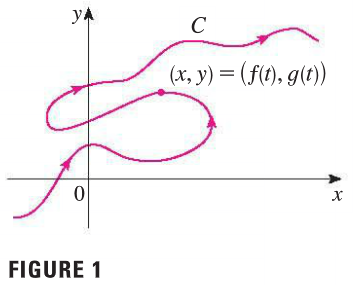
\includegraphics[scale=0.45]{10-1pic1.png}\]

\indent\\

Imagine that a particle moves along the curve $C$ shown in Figure 1. It is IMPOSSIBLE to describe $C$ by an equation of the form $y=f(x)$ because $C$ fails the \underline{\hspace{1in}} \underline{\hspace{0.75in}} Test.\\
\indent

But the $x-$ and $y-$coordinates of the particle are functions of time and so we can write \underline{\hspace{1.25in}} and \underline{\hspace{1.25in}}. Such a pair of equations is often a convenient way of describing a curve and gives rise to the following definition.\\
\indent\\
\indent\\
\indent\\

\fbox{
  \parbox{\textwidth}{
  \vspace{5pt} \underline{\textbf{Definition:}} \\
  \indent
  
  Suppose that $x$ and $y$ are both given as functions of a third variable $t$ (called a \textbf{parameter}) by the equations
  \[x=f(t) \quad \text{ and } \quad y=g(t)\]
  
  (called \textbf{parametric equations}). Each value of $t$ determines a point $(x,y)$, which we can plot in a coordinate plane. As $t$ varies, the point\\
  \[(x,y) = (f(t),g(t))\]
  \indent
  
  varies and traces out a curve $C$, which we call a \underline{\hspace{1.5in}} \underline{\hspace{1in}}.\\
  \indent
  
  }}
  \indent\\
  \indent
  

  
  \underline{Example 1}: Sketch and identify the curve defined by the parametric equations
  \[x=t^2 - 2t \quad \quad y=t+1\]
 
 SOLUTION:\\
 
 
 \vspace{3in}
 
 *Notice that the consecutive points marked on the curve appear at equal time intervals but not at equal distances. That is because the particle slows down and then speeds up as $t$ increases. \\
 
 
 \vspace{2in}
 
 Thus, the curve represented by the given parametric equation is the \underline{\hspace{1in}} \underline{\hspace{1.9in}}.\\
 \indent\\
 \indent
 \vspace{0.5in}
 
 In general:\\

\begin{itemize}
 \item We call the equation of a curve in terms of $x$ and $y$, the \underline{\hspace{1.25in}} \underline{\hspace{1in}}.\\
 \item We call the equation of a curve with $x$ and $y$ given in terms of a parameter (such as $t$) the \underline{\hspace{1.25in}} \underline{\hspace{1in}}.
 \end{itemize}
 
 \underline{Note}: No restriction was placed on the parameter $t$ in Example 1, so we assumed that $t$ could be any real number. But sometimes we restrict $t$ to lie in a finite interval. For instance, the parametric curve
 \[x=t^2-2t \quad \quad y=t+1 \quad \quad 0\leq t\leq 4\]
 shown below is the part of the parabola in Example 1 that starts at the point $(0,1)$ and ends at the point $(8,5)$. The arrowhead indicates the direction in which the curve is traced as $t$ increases from 0 to 4.\\
 \[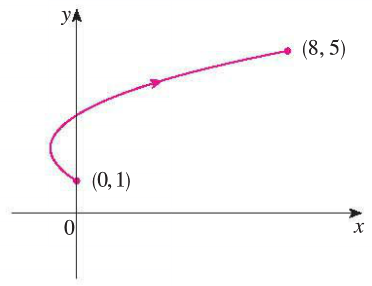
\includegraphics[scale=0.45]{10-1pic2.png}\]
 
 In general, the curve with parametric equations
 \[x=f(t) \quad \quad y=g(t) \quad \quad a\leq t\leq b\]
 has \textbf{initial point} $(f(a),g(a))$ and \textbf{terminal point} $(f(b),g(b))$.\\
 \indent\\
 \indent
 
 \underline{Example 2}: What curve is represented by the following parametric equations?
 \[x=\cos t \quad \quad y=\sin t \quad \quad 0 \leq t \leq 2\pi\]
 \indent
 
 SOLUTION:\\
 
 \vspace{4in}
 
 \newpage
 
 \underline{Example 3}: What curve is represented by the given parametric equations?
 \[x=\sin 2t \quad \quad y=\cos 2t \quad \quad 0\leq t\leq 2\pi\]
 \indent
 
 SOLUTION: Again we have
 
 \vspace{0.5in}
 
 so the parametric equations again represent the unit circle $x^2+y^2=1$. But as $t$ increases from $0$ to $2\pi$, the point $(x,y)=(\sin 2t, \cos 2t)$ starts at $(0,1)$ and moves \textit{twice} around the circle in the clockwise directions as see here:
 
 \[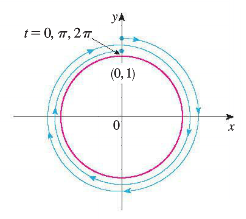
\includegraphics[scale=0.6]{10-1pic3.png}\]
 
 \vspace{0.15in}
 
 \underline{Example 4}: Find parametric equations for the circle with center $(h,k)$ and radius $r$.\\
 \indent
 
 SOLUTION:\\
 
 \vspace{2.75in}
  \newpage
 \[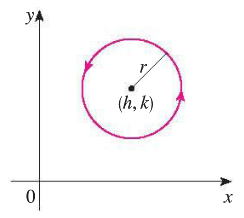
\includegraphics[scale=0.45]{10-1pic4.png}\]
 \indent

 \underline{Example 5}: Sketch the curve with parametric equations $x=\sin t$, $y=\sin^2 t$.\\
 \indent
 
 SOLUTION:\\
 \indent
 
 \vspace{2in}
 
% \[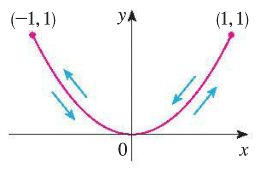
\includegraphics[scale=0.45]{10-1pic5.png}\]
 \indent
 
 %The importance or usefulness of paramtric curves with CAD and graphical images
 
% \section*{The Cycloid}
% 
% \underline{Example 7}: The curve traced out by a point $P$ on the circumference of a circle as the circle rolls along a straight line is called a \underline{\hspace{1in}}.
% \[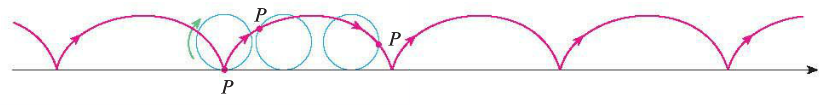
\includegraphics[scale=0.45]{10-1pic6.png}\]
% 
% If the circle has radius $r$ and rolls along the $x-$axis and if one position of $P$ is the origin, find parametric equations for the cycloid.\\
% \indent
% 
% SOLUTION:\\
% \indent
 
 
 
 %not finished
 
% \section*{Families of Parametric Curves}
% \underline{Example 8}: Investigate the family of curves with parametric equations
% \[x=a + \cos t \quad \quad y=a\tan t + \sin t\]
% What do these curves have in common? How does the shape change as $a$ increases?\\
% \indent
% 
% SOLUTION:\\
% \indent
 
 
 
 

%\fbox{
%  \parbox{\textwidth}{
%  \vspace{5pt}

%----------------------------------------------------------------------------------------

\end{document}